
\documentclass[conference]{IEEEtran}

\usepackage[pdftex]{graphicx}
\graphicspath{ {../images/} }
\usepackage{caption}
\usepackage{subfigure}
\usepackage{float}

\usepackage{hyperref}
\hypersetup
{
    colorlinks=true,
    linkcolor=black,   
    urlcolor=blue,
    citecolor=black,
}

% *** ALIGNMENT PACKAGES ***
%
%\usepackage{array}
% Frank Mittelbach's and David Carlisle's array.sty patches and improves
% the standard LaTeX2e array and tabular environments to provide better
% appearance and additional user controls. As the default LaTeX2e table
% generation code is lacking to the point of almost being broken with
% respect to the quality of the end results, all users are strongly
% advised to use an enhanced (at the very least that provided by array.sty)
% set of table tools. array.sty is already installed on most systems. The
% latest version and documentation can be obtained at:
% http://www.ctan.org/tex-archive/macros/latex/required/tools/


%\usepackage{mdwmath}
%\usepackage{mdwtab}
% Also highly recommended is Mark Wooding's extremely powerful MDW tools,
% especially mdwmath.sty and mdwtab.sty which are used to format equations
% and tables, respectively. The MDWtools set is already installed on most
% LaTeX systems. The lastest version and documentation is available at:
% http://www.ctan.org/tex-archive/macros/latex/contrib/mdwtools/


% IEEEtran contains the IEEEeqnarray family of commands that can be used to
% generate multiline equations as well as matrices, tables, etc., of high
% quality.


% *** SUBFIGURE PACKAGES ***
%\usepackage[tight,footnotesize]{subfigure}
% subfigure.sty was written by Steven Douglas Cochran. This package makes it
% easy to put subfigures in your figures. e.g., "Figure 1a and 1b". For IEEE
% work, it is a good idea to load it with the tight package option to reduce
% the amount of white space around the subfigures. subfigure.sty is already
% installed on most LaTeX systems. The latest version and documentation can
% be obtained at:
% http://www.ctan.org/tex-archive/obsolete/macros/latex/contrib/subfigure/
% subfigure.sty has been superceeded by subfig.sty.


% *** FLOAT PACKAGES ***
%
%\usepackage{fixltx2e}
% fixltx2e, the successor to the earlier fix2col.sty, was written by
% Frank Mittelbach and David Carlisle. This package corrects a few problems
% in the LaTeX2e kernel, the most notable of which is that in current
% LaTeX2e releases, the ordering of single and double column floats is not
% guaranteed to be preserved. Thus, an unpatched LaTeX2e can allow a
% single column figure to be placed prior to an earlier double column
% figure. The latest version and documentation can be found at:
% http://www.ctan.org/tex-archive/macros/latex/base/



%\usepackage{stfloats}
% stfloats.sty was written by Sigitas Tolusis. This package gives LaTeX2e
% the ability to do double column floats at the bottom of the page as well
% as the top. (e.g., "\begin{figure*}[!b]" is not normally possible in
% LaTeX2e). It also provides a command:
%\fnbelowfloat
% to enable the placement of footnotes below bottom floats (the standard
% LaTeX2e kernel puts them above bottom floats). This is an invasive package
% which rewrites many portions of the LaTeX2e float routines. It may not work
% with other packages that modify the LaTeX2e float routines. The latest
% version and documentation can be obtained at:
% http://www.ctan.org/tex-archive/macros/latex/contrib/sttools/
% Documentation is contained in the stfloats.sty comments as well as in the
% presfull.pdf file. Do not use the stfloats baselinefloat ability as IEEE
% does not allow \baselineskip to stretch. Authors submitting work to the
% IEEE should note that IEEE rarely uses double column equations and
% that authors should try to avoid such use. Do not be tempted to use the
% cuted.sty or midfloat.sty packages (also by Sigitas Tolusis) as IEEE does
% not format its papers in such ways.

% correct bad hyphenation here
\hyphenation{op-tical net-works semi-conduc-tor}

%\usepackage[style=numeric,sorting=none]{biblatex}
%\addbibresource{roco318.bib}

\begin{document}
%
% paper title
% can use linebreaks \\ within to get better formatting as desired
\title{AINT308 - Machine Vision and Behavioural Computing\\Coursework 1 Report}


% author names and affiliations
% use a multiple column layout for up to three different
% affiliations
\author{\IEEEauthorblockN{Student No. 10613591}
\IEEEauthorblockA{School of Engineering,\\Computing and Mathematics
\\University of Plymouth\\
Plymouth, Devon}}



% make the title area
\maketitle


\begin{abstract}
%\boldmath
 Machine Vision is field of study who's applications are becoming rapidly more prevalent amongst contemporary technology, with advancements having large implications in a wide variety of fields. This report details the use of a popular open-source machine vision library, \textbf{OpenCV}, in three different applications: Identifying the most common colour in an image, tracking a moving object within a video, and matching sub-components of an image to a larger image.
\end{abstract}
\subsection*{Keywords:}
Machine Vision, OpenCV, Object Tracking

\section{Task 1 - Colour Sorter}
\subsection{Introduction}
The first task involves creating a system able to label a dataset of car colours reg, green, or blue.
\subsection{Solution}
As part of its suite of features, \textbf{OpenCV} includes the ability to retrieve individual pixel's values. The specific values available will vary based on the colour space used. For example, working in the \textit{RGB} colour space enables a pixel's \textit{Red,Green} and \textit{Blue} values to be retrieved. Using this information, it is possible to calculate the mode colour of an image. 

\begin{figure}[H]
\centering
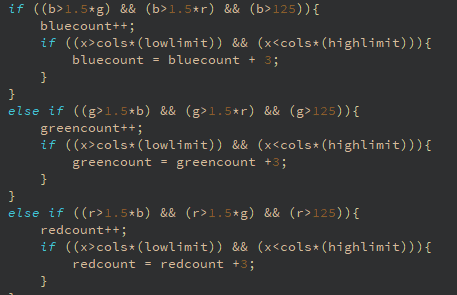
\includegraphics[width=2.5in]{t1}
\caption{Pixel testing code}
\label{fig_t1code}
\end{figure}

The code in figure \ref{fig_t1code} performs the checks needed to assertain a pixel's primary colour. Initial attempts simply checked which of three component values were highest. In practice, this method was inaccurate as it had no way between differentiating between a near-white cell (such as a background cloud) which would have near equal \textit{RGB} values, and one that belonged to the subject (in this case, the car).

To allow the algorithm to differentiate between background elements and the subject, two methods were employed. Firstly, a pixel was only counted if that colour's value was a significant margin higher than the other values. In figure \ref{fig_t1code} this margin is $50\%$. Additionally, the pixel's value must be greater than half the colour space's maximum value, in this case 125. This prevents background objects from being counted.


Additionally, extra weighting is applied to pixels within a central rectangle on the screen. This area can be changed by editing the values $highlimit$ and $lowlimit$. By adding this additional weighting to central areas, background areas are further discounted, helping to prevent false positives by valuing true positives more.

With the provided testing dataset of thirty red, blue, or green cars this solution is 100$\%$ accurate, correctly identifying the subject's colour in every image. This is a marked improvement from the simple method used in the initial attempt, which would often get confused at reflections in windows (these would be reflecting the sky, which would add bias towards blue), background walls (especially brick, which would bias the results towards red), and any natural backgrounds (adding green bias).

\subsection{Limitations}
This solution is extremely limited
\subsection{Further Improvements}
\subsection{Conclusion}

\section{Task 2 - Object Tracking}
\subsection{Introduction}
\subsection{Solution}
\subsection{Limitations}
\subsection{Further Improvements}
\subsection{Conclusion}

\section{Task 3 - Image Mapping}
\subsection{Introduction}
\subsection{Solution}
\subsection{Limitations}
\subsection{Further Improvements}
\subsection{Conclusion}


% An example of a floating figure using the graphicx package.
% Note that \label must occur AFTER (or within) \caption.
% For figures, \caption should occur after the \includegraphics.
% Note that IEEEtran v1.7 and later has special internal code that
% is designed to preserve the operation of \label within \caption
% even when the captionsoff option is in effect. However, because
% of issues like this, it may be the safest practice to put all your
% \label just after \caption rather than within \caption{}.
%
% Reminder: the "draftcls" or "draftclsnofoot", not "draft", class
% option should be used if it is desired that the figures are to be
% displayed while in draft mode.
%
%\begin{figure}[H]
%\centering
%\includegraphics[width=2.5in]{myfigure}
% where an .eps filename suffix will be assumed under latex, 
% and a .pdf suffix will be assumed for pdflatex; or what has been declared
% via \DeclareGraphicsExtensions.
%\caption{Simulation Results}
%\label{fig_sim}
%\end{figure}

% Note that IEEE typically puts floats only at the top, even when this
% results in a large percentage of a column being occupied by floats.


% An example of a double column floating figure using two subfigures.
% (The subfig.sty package must be loaded for this to work.)
% The subfigure \label commands are set within each subfloat command, the
% \label for the overall figure must come after \caption.
% \hfil must be used as a separator to get equal spacing.
% The subfigure.sty package works much the same way, except \subfigure is
% used instead of \subfloat.
%
%\begin{figure*}[!t]
%\centerline{\subfloat[Case I]\includegraphics[width=2.5in]{subfigcase1}%
%\label{fig_first_case}}
%\hfil
%\subfloat[Case II]{\includegraphics[width=2.5in]{subfigcase2}%
%\label{fig_second_case}}}
%\caption{Simulation results}
%\label{fig_sim}
%\end{figure*}
%
% Note that often IEEE papers with subfigures do not employ subfigure
% captions (using the optional argument to \subfloat), but instead will
% reference/describe all of them (a), (b), etc., within the main caption.


% An example of a floating table. Note that, for IEEE style tables, the 
% \caption command should come BEFORE the table. Table text will default to
% \footnotesize as IEEE normally uses this smaller font for tables.
% The \label must come after \caption as always.
%
%\begin{table}[!t]
%% increase table row spacing, adjust to taste
%\renewcommand{\arraystretch}{1.3}
% if using array.sty, it might be a good idea to tweak the value of
% \extrarowheight as needed to properly center the text within the cells
%\caption{An Example of a Table}
%\label{table_example}
%\centering
%% Some packages, such as MDW tools, offer better commands for making tables
%% than the plain LaTeX2e tabular which is used here.
%\begin{tabular}{|c||c|}
%\hline
%One & Two\\
%\hline
%Three & Four\\
%\hline
%\end{tabular}
%\end{table}


% Note that IEEE does not put floats in the very first column - or typically
% anywhere on the first page for that matter. Also, in-text middle ("here")
% positioning is not used. Most IEEE journals/conferences use top floats
% exclusively. Note that, LaTeX2e, unlike IEEE journals/conferences, places
% footnotes above bottom floats. This can be corrected via the \fnbelowfloat
% command of the stfloats package.


\newpage
\appendix

%\printbibliography


% that's all folks
\end{document}